\chapter{Risultati e confronto}
In questo capitolo si confrontano i risultati di simulazioni eseguite con differenti schemi si risoluzione.
\section{Soluzione Analitica del Pendolo Semplice}
Al fine di stimare l'entità dell'errore dei metodi proposti è necessario confrontare i risultati ottenuti con una soluzione analitica. Un tipico problema di meccanica vincolata per il quale esiste una soluzione analitica è il pendolo semplice. Si prende in considerazione il caso generale, ossia \textbf{non} si assume $sin\theta \sim \theta$

Seguendo la soluzione proposta in \cite{Davis} per conoscere l'angolo $\theta$ e la sua derivata rispetto al tempo, la velocità angolare $\dot{\theta}$ si procede come segue:
\begin{figure}[h!]
\centering
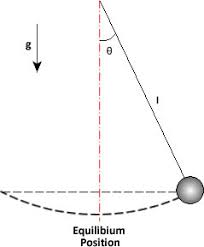
\includegraphics[height=5cm]{Figure/pend.jpg}
\caption{Schema di un pendolo semplice}
 \label{fig:Pend}
\end{figure}
Si consideri innanzitutto il principio della conservazione dell'energia, che in questo caso consta di 2 termini, uno cinetico ed uno gravitazionale. Pertanto, dato un angolo di partenza $\theta_0$ con velocità iniziale nulla si, si può scrivere:
\begin{equation}
    mgl\left(1-cos\theta_0\right) = mgl\left(1-cos\theta \right)+\frac{1}{2}I\dot{\theta}^2
\end{equation}
Da cui:
\begin{equation}
    \dot{\theta} = \sqrt{\frac{2mgl}{I}} \sqrt{cos\theta - cos\theta_0}
\end{equation}
\begin{equation}
    dt =  \sqrt{\frac{I}{2mgl}} \frac{d\theta}{\sqrt{cos\theta - cos\theta_0}} 
\end{equation}
Per integrare il termine in $\theta$ si introduce la sostituzione:
\begin{equation} \label{eq:pend_sub}
    cos\theta = 1-2k^2sin^2\Phi \quad ; \qquad k = sin\frac{\theta_0}{2}
\end{equation}

Si osserva che che:
\begin{align} \nonumber
cos\theta - cos\theta_0 &=  1-2k^2sin^2\Phi - cos\theta_0  \\ \nonumber
&= 1-2k^2(1-cos^2\Phi) - cos\theta_0 \\ \nonumber
&= 1-2k^2+2k^2cos^2\Phi-cos\theta_0 \\ \nonumber
\left( k = sin\frac{\theta_0}{2}, cos\theta = 1-2sin^2\frac{\theta}{2}\right) \rightarrow &=cos\theta_0+ 2k^2cos^2\Phi - cos\theta_0 \\
cos\theta - cos\theta_0 &= 2k^2cos^2\Phi
\end{align}

\begin{align}
    sin\theta &= \sqrt{1-2cos^2\theta} \\ \nonumber
    &= \sqrt{1-(1-2k^2sin^2\Phi} \\ \nonumber
    &= \sqrt{1-(1+4k^4sin^4\Phi-4k^2sin^2\Phi)} \\ \nonumber
    &= \sqrt{4k^2sin^2\Phi - 4k^4sin^4\Phi} \\ \nonumber
    &= \sqrt{4k^2sin^2\Phi(1-k^2sin^2\Phi} \\
    sin\theta &= 2ksin\Phi\sqrt{(1-k^2sin^2\Phi)}  \
\end{align}

\begin{equation}
    sin\theta d\theta = 2k^2sin\Phi cos\Phi d\Phi
\end{equation}

Utilizzando queste relazioni partendo da \ref{eq:pend_sub} si può ottenere: 
\[\sqrt{\frac{I}{2mgl}} \frac{d\theta}{\sqrt{cos\theta - cos\theta_0}} = \sqrt{\frac{I}{2mgl}} 
\frac{sin\theta d\theta}{sin\theta\sqrt{cos\theta - cos\theta_0}} = \]
\[
= \sqrt{\frac{I}{2mgl}} \frac{4k^2sin\Phi cos\Phi d\Phi}{2ksin\Phi\sqrt{(1-k^2sin^2\Phi)} \sqrt{2k^2cos^2\Phi} } 
\]
Ed infine:
\begin{equation} \label{eq:pend_diff}
    dt = \sqrt{\frac{I}{mgl}} \frac{d\Phi}{\sqrt{1-k^2sin^\Phi}} 
\end{equation}
Integrando la \ref{eq:pend_diff} si ottiene un integrale ellittico incompleto del primo tipo:
\begin{equation} \label{eq:pend_int}
    t = \sqrt{\frac{I}{mgl}}  \int_0^\Phi \frac{d\Phi}{\sqrt{1-k^2sin^\Phi}}
\end{equation}
Ricordando che la funzione ellittica di Jacobi è definita come l'inverso dell'integrale ellittico del primo tipo, ossia dato:
\begin{equation}
    u =  \int_0^\Phi \frac{d\Phi}{\sqrt{1-k^2sin^\Phi}}
\end{equation}

\begin{equation} \label{eq:JacobiSN}
    sn(u|k) = sin(\Phi) \qquad cn(u|k) = cos(\Phi) \qquad dn(u|k) = \sqrt{1-k^2sin^\Phi}
\end{equation}

Per cui, utilizzando la prima relazione di \ref{eq:JacobiSN} \newline e ricordando che \( cos\theta = 1-2sin^2\left(\frac{\theta}{2}\right) \)
\begin{equation}
    sn\left( \sqrt{\frac{mgl}{I}t} \quad | \quad k \right) = sin(\Phi) = \frac{1}{k}sin\left(\frac{\theta}{2}\right)
\end{equation}
Infine si ottiene:
\begin{align}
    \theta &= 2 arcsin \left[ k \quad sn\left( \sqrt{\frac{mgl}{I}t} \quad | \quad k \right)   \right] 
    \\ \nonumber  k &= sin\frac{\theta_0}{2}
\end{align}

\subsection{Relative Percent Difference}
%Prossimità dello zero che dipende da sfiga 'punti vicini porta esempio trapz
Nella stima dell'accuratezza di un metodo si dovrà tenere conto di due fattori: innanzitutto ogni metodo è ovviamente esatto nelle condizioni iniziali, ad andrà via via allontanandosi dalla soluzione esatta. Per questa ragione si è considerata la media dell'errore su due oscillazioni complete per avere un dato più significativo dell'accuratezza del metodo.

Bisogna inoltre tener presene che entrambi i valori (analitico e numerico) possono annullarsi. Questo può portare a sovrastimare l'errore relativo, come appare evidente in figura \ref{fig:HHT_relerr}: la soluzione numerica è praticamente sempre sovrapposta a quella analitica, ma in prossimità di x=0 l'errore relativo diventa estremamente elevato. È quindi consigliabile non utilizzare l'errore relativo. Si potrebbe utilizzare la formula della differenza relativa che utilizza il valor medio per scalare il risultato. 

\begin{equation}
    rd = \frac{(|v_{an}| - |v_{approx}|)}  { \frac{|v_{an}| + |v_{approx}|}{2}  }
\end{equation}

Dove $v_an$ e $v_approx$ sono rispettivamente il valore analitico e l'approssimazione numerica che si vuole confrontare.

Questo accorgimento limita il sovracitato problema come visibile in figura \ref{fig:HHT_relerr}, tuttavia quando uno dei due valori si annulla essa vale 2 \textbf{indipendentemente} dalla bontà dell'approssimazione. Per questa ragione si è scelto di non utilizzare nessuna scalatura dell'errore. Si utilizza semplicemente la media dei valori assoluti dell'errore \ref{eq:mean_err} per valutare la convergenza dell'algoritmo.
\begin{equation}
    \label{eq:mean_err}
    e_{mean} = \sum_{i=0}^{i=N} |v_{i, an} - v_{i, approx}|
\end{equation}

\begin{figure}[h!]
\centering
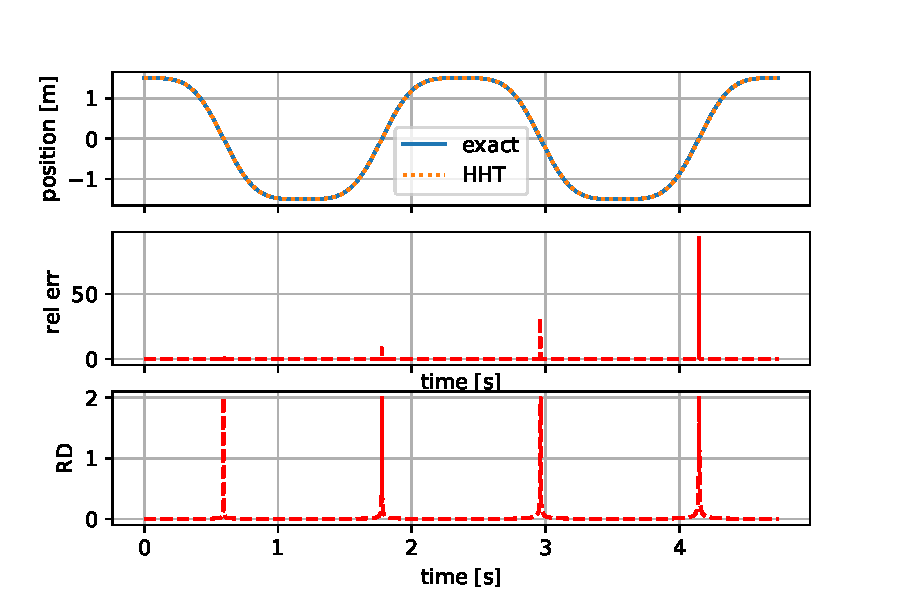
\includegraphics[height=7cm]{Figure/HHT_relerr.pdf}
\caption{Metodo HHT timestep = 5E-4}
 \label{fig:HHT_relerr}
\end{figure}

\section{Verifica Numerica della convergenza}
% andamento posizione all'infittire di h (poco), 
%andamento somma errori con h (importante perchè mostra convergenza
%parametri (se presenti)
In questa sezione vengono confrontati i risultati numerici al variare dell'ampiezza del timestep con la soluzione analitica. Si verifica che al ridursi del timestep l'errore medio \ref{eq:mean_err} tenda a zero.

Inoltre si confrontano le posizioni della punta del pendolo per visualizzare graficamente il risultato dell'integrazione numerica.
\subsection{Eulero Implicito}
Presenta il maggior smorzamento numerico, inoltre anche per timestep relativamente brevi si discosta (0.01s) si discosta visibilmente dalla soluzione esatta. 
Al tendere del timestep a $10^{-4}$, tuttavia, l'errore tende rapidamente a 0.


\begin{figure}[h!]
\centering
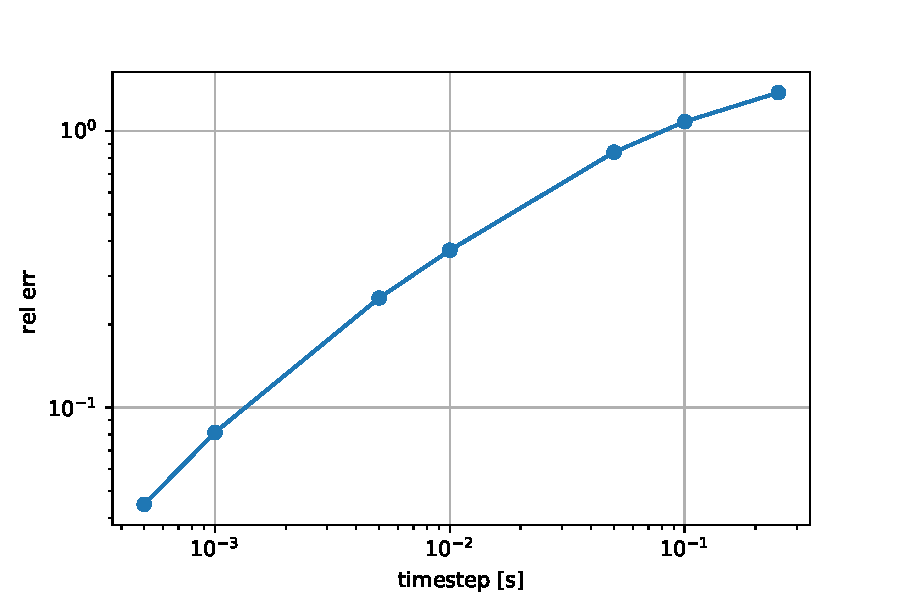
\includegraphics[height=7cm]{Figure/Convergenza/EulImp_err.pdf}
\caption{Convergenza del metodo di Eulero implicito}
 \label{fig:EulImp_err}
\end{figure}

\begin{figure}[h!]
\centering
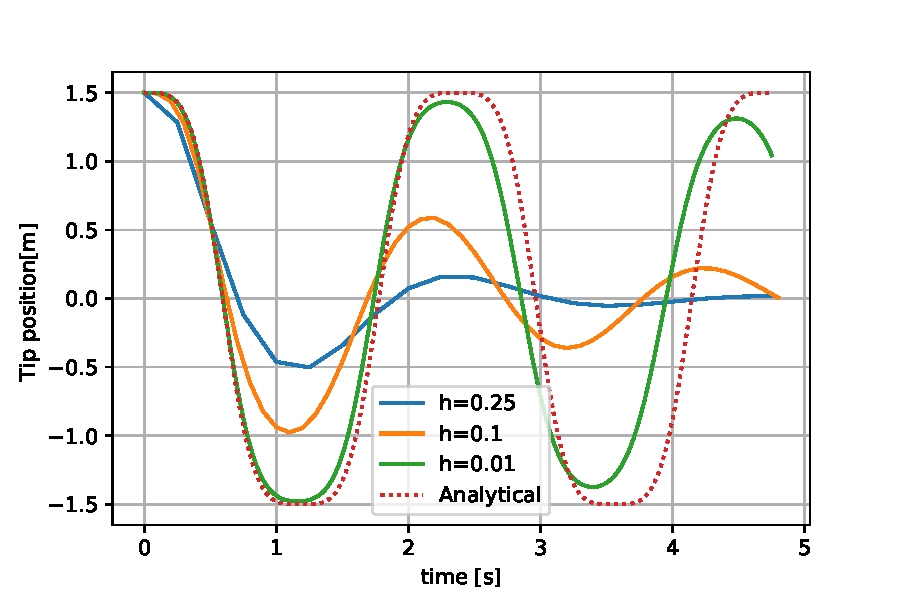
\includegraphics[height=7cm]{Figure/Convergenza/EulImp_pos.pdf}
\caption{Grafico posizione metodo di Eulero implicito}
 \label{fig:EulImp_pos}
\end{figure}
\FloatBarrier
\subsection{Metodo dei Trapezi}
Rispetto al metodo di Eulero implicito lo smorzamento numerico è minore e per timestep pari a 0.01s la soluzione è relativamente vicina a quella esatta.
\begin{figure}[h!]
\centering
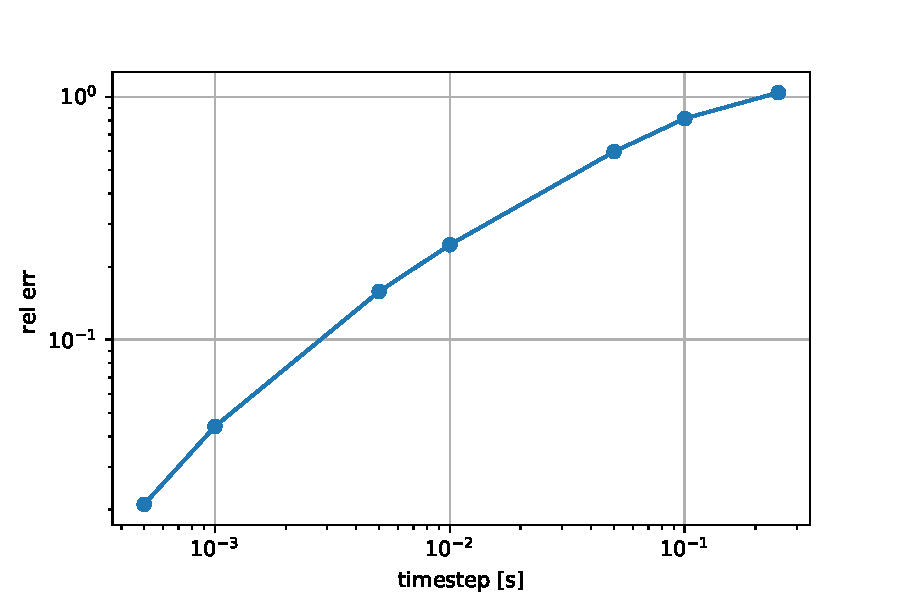
\includegraphics[height=7cm]{Figure/Convergenza/Trapz_err.pdf}
\caption{Convergenza del metodo dei trapezi}
 \label{fig:Trapz_err}
\end{figure}

\begin{figure}[h!]
\centering
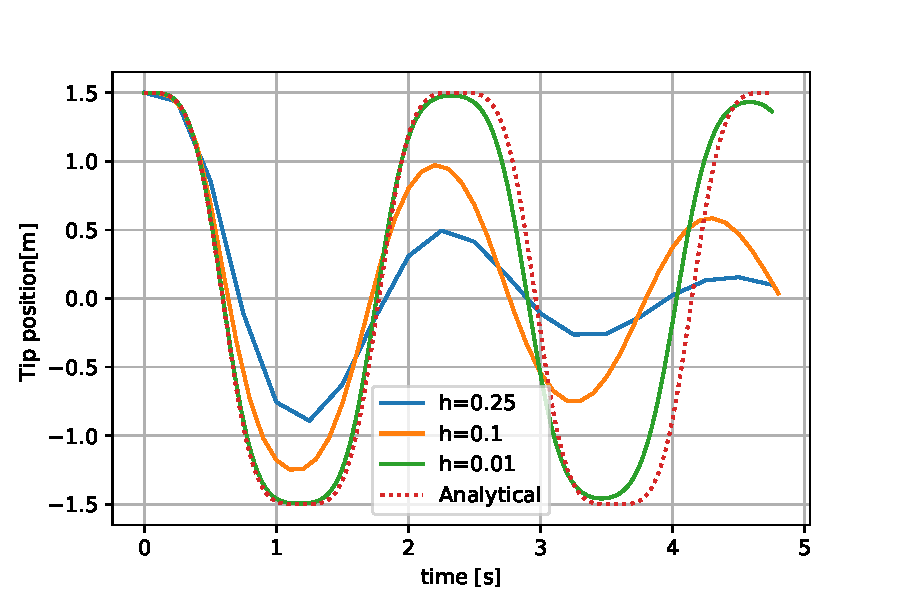
\includegraphics[height=7cm]{Figure/Convergenza/Trapz_pos.pdf}
\caption{Grafico posizione del metodo dei trapezi}
 \label{fig:Trapz_pos}
\end{figure}
\FloatBarrier
\subsection{Metodo di Newmark}
Il metodo di Newmark presenta un'elevata instabilità per timestep elevati, al punto che per $ts > 0.05$ la soluzione diverge. Poiché l'errore medio di questi casi schiaccerebbe il grafico, si riportano i risultati per $ts < 0.05$.
Nonostante il problema elencato questo metodo presenta un'ottima approssimazione e come si nota dalla figura \ref{fig:Trapz_pos} già per $ts = 0.025$ l'approssimazione si sovrappone alla soluzione esatta.
\begin{figure}[h!]
\centering
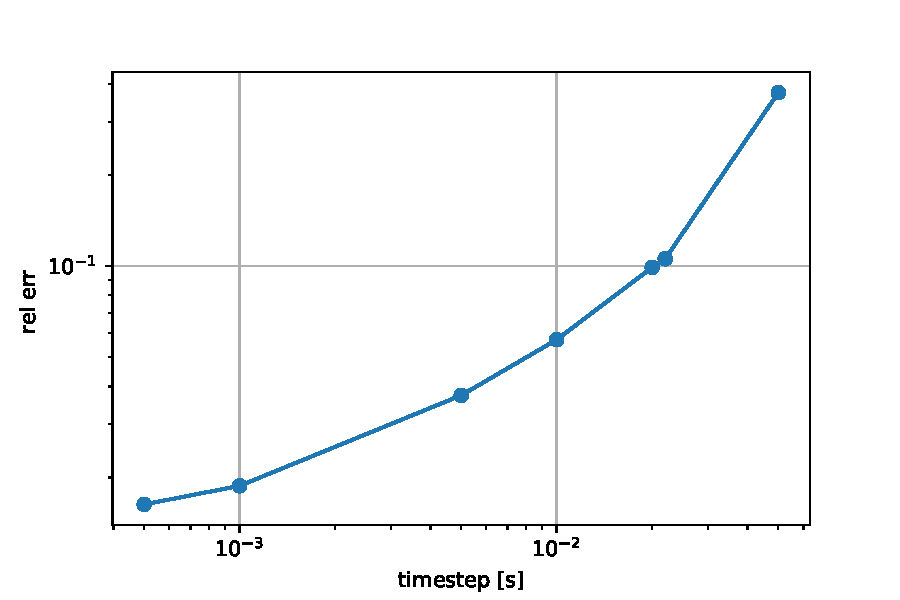
\includegraphics[height=7cm]{Figure/Convergenza/Newm.pdf}
\caption{Convergenza del metodo di Newmark}
 \label{fig:Newm}
\end{figure}

\begin{figure}[h!]
\centering
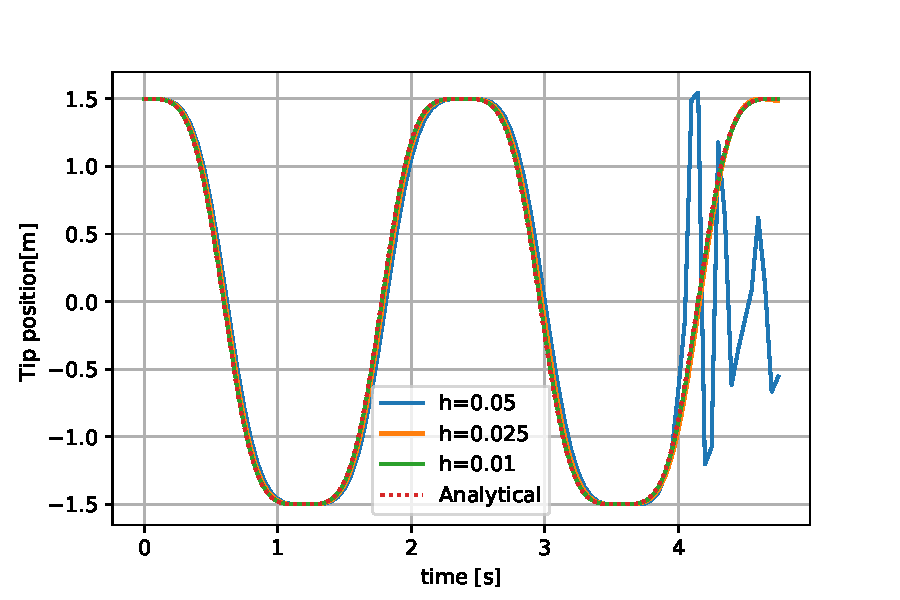
\includegraphics[height=7cm]{Figure/Convergenza/Newm_pos.pdf}
\caption{Grafico posizione del metodo di Newmark}
 \label{fig:Newm_pos}
\end{figure}
\FloatBarrier
\paragraph{Tuning dei Parametri}
Il metodo di Newmark presenta ordine 2 solo per $\gamma = 1/2$, per il quale inoltre lo smorzamento numerico è nullo. Per questa ragione ci si limita ad indagare gli effetti della variazione di $\beta$, tenendo $\gamma = 1/2$. Si ricorda che la condizione di assoluta stabilità è $\beta \geq \frac{(\gamma + \frac{1}{2})^2}{4}$, per cui per $\gamma = 1/2$ il metodo è assolutamente stabile per $\beta \geq 1/4$. Utilizzando la accelerazione lineare ($\beta = 1/6$) si esce dalla assoluta stabilità ed infatti la simulazione diverge. Variando $\beta$ nella regione di assoluta stabilità si ottiene invece che se esso è leggermente maggiore di quanto prescritto dalla condizione (0.27 invece di 0.25, come visibile in \ref{fig:NewmComp}) ne beneficia la stabilità per timestep più elevati senza inficiare la bontà dell'approssimazione per timestep ridotti.

\begin{figure}[h!]
\centering
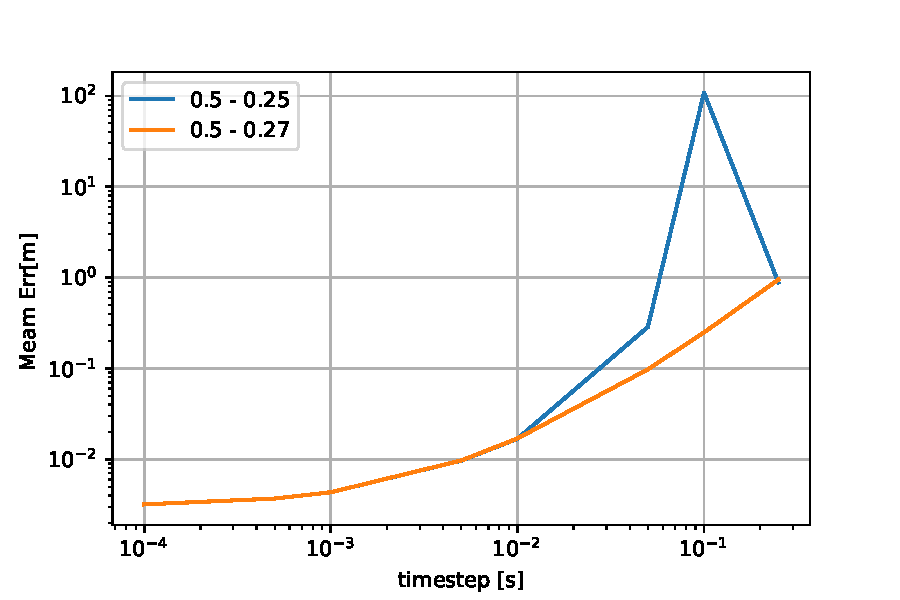
\includegraphics[height=7cm]{Figure/Convergenza/NewmComp.pdf}
\caption{Convergenza del metodo HHT}
 \label{fig:NewmComp}
\end{figure}

\FloatBarrier
\subsection{Metodo HHT}

\begin{figure}[h!]
\centering
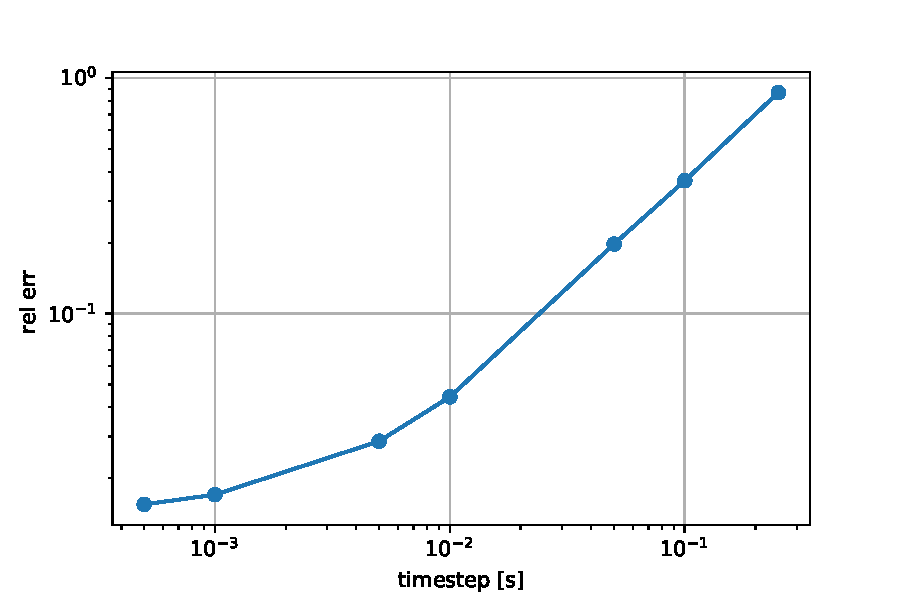
\includegraphics[height=7cm]{Figure/Convergenza/HHT_err.pdf}
\caption{Convergenza del metodo HHT}
 \label{fig:HHT_err}
\end{figure}

\begin{figure}[h!]
\centering
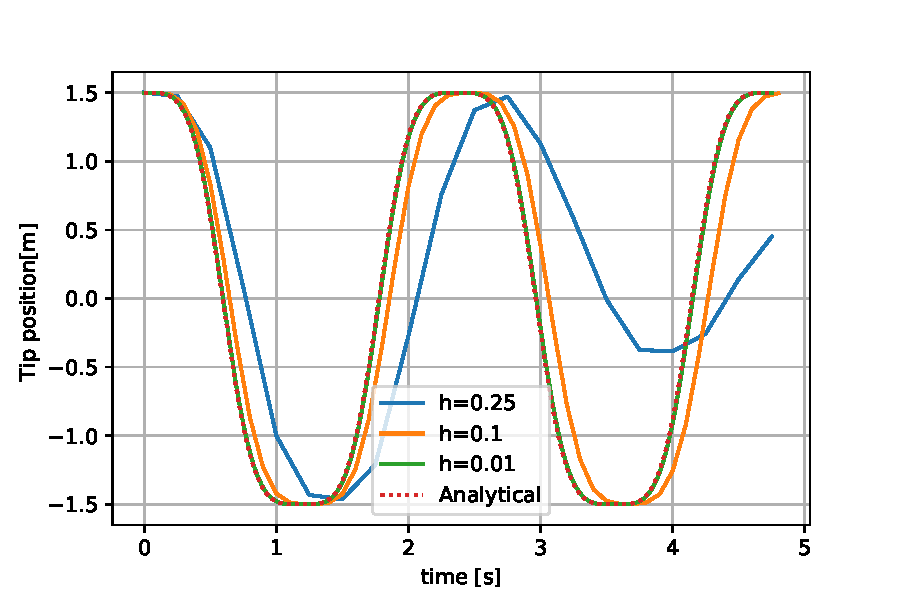
\includegraphics[height=7cm]{Figure/Convergenza/HHT_pos.pdf}
\caption{Grafico posizione del metodo HHT}
 \label{fig:HHT_pos}
\end{figure}
\FloatBarrier

\paragraph{Tuning dei Parametri}
Come accennato in precedenza ponendo $\alpha=0$ ed ottenendo $\beta$ e $\gamma$ a partire da $\alpha$ come suggerito si ottiene il metodo di Newmark con accelerazione costante, e presenta gli stessi problemi di stabilità per timestep più lunghi \ref{fig:HHTComp}. Aumentando $\alpha$ cresce lo smorzamento numerico, ma al contempo il metodo diventa stabile. Si nota che (come anche noto dalla letteratura) il miglior valore di $\alpha$ è il più piccolo valore che permette la convergenza come visibile in \ref{fig:HHTComp2}.
\begin{figure}[h!]
\centering
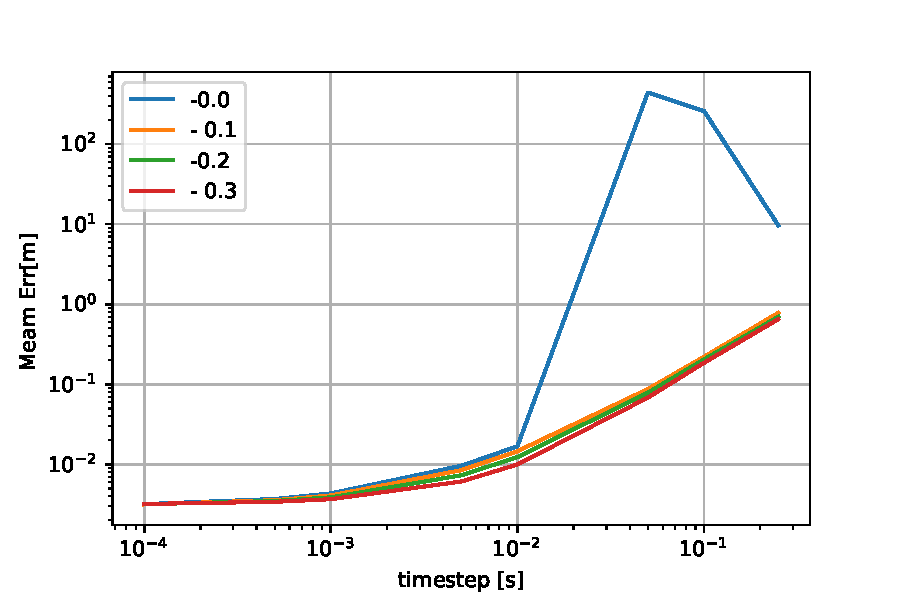
\includegraphics[height=7cm]{Figure/Convergenza/HHTComp.pdf}
\caption{Errore del metodo HHT al variare di $\alpha$}
 \label{fig:HHTComp}
\end{figure}
\begin{figure}[h!]
\centering
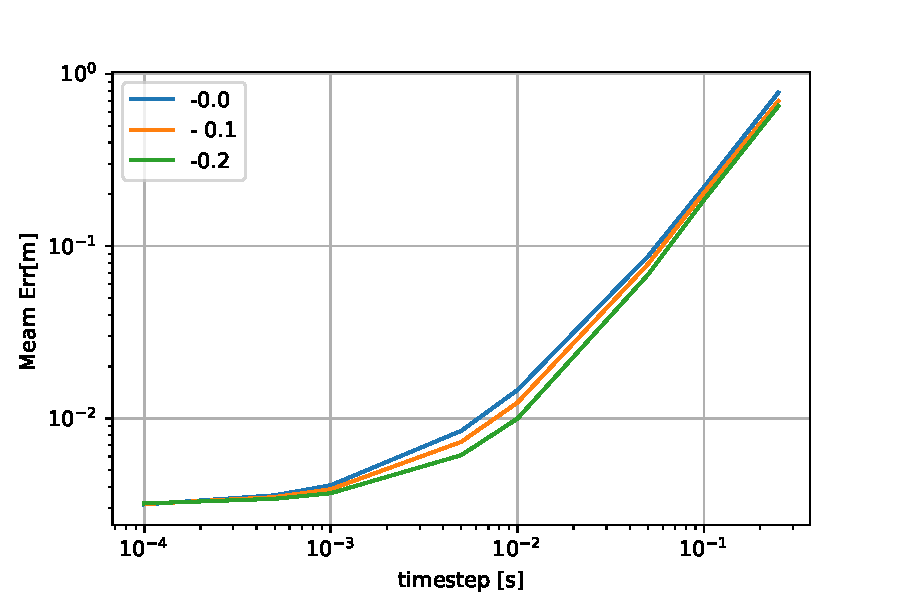
\includegraphics[height=7cm]{Figure/Convergenza/HHTComp2.pdf}
\caption{Errore del metodo HHT al variare di $\alpha$}
 \label{fig:HHTComp2}
\end{figure}
\FloatBarrier
\section{Confronto fra i metodi}
I metodi ad hoc offrono performance migliori, osservando i grafici in figura \ref{fig:ErrComp} ed il particolare per timestep ridotti \ref{fig:ErrComp_zoom}. 

Si nota che per timestep relativamente ampi (anche 0.1) il metodo HHT giunge a buone approssimazioni, ed in particolare per $ts \sim 0.01$, ovvero i tipici valori del timestep usati nella simulazioni multibody, l'approssimazione di HHT e Newmark è molto buona e ridotta rispetto ai metodi generici.
\begin{figure}[h!]
\centering
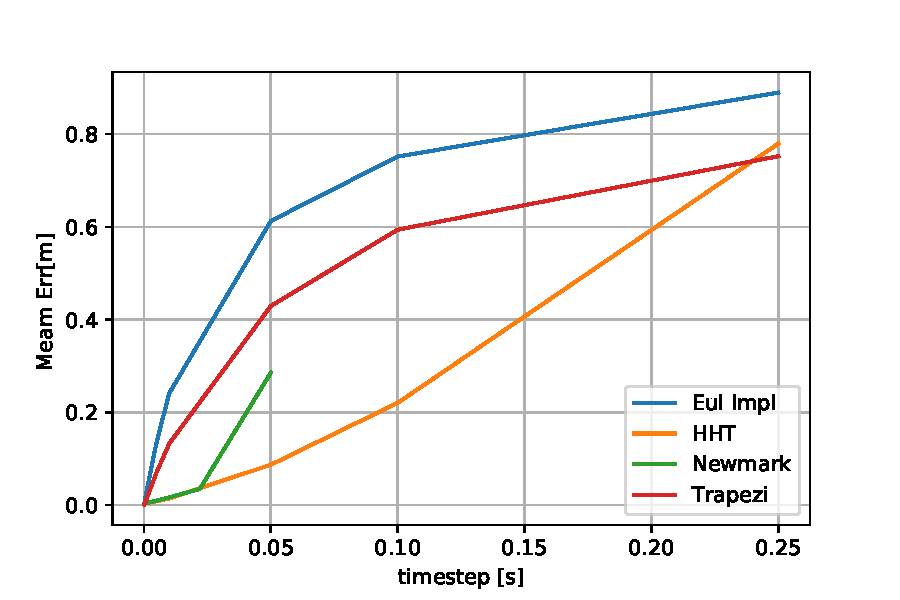
\includegraphics[height=7cm]{Figure/Convergenza/ErrComp.pdf}
\caption{Confronto Errore Medio Metodi Integrazione}
 \label{fig:ErrComp}
\end{figure}

\begin{figure}[h!]
\centering
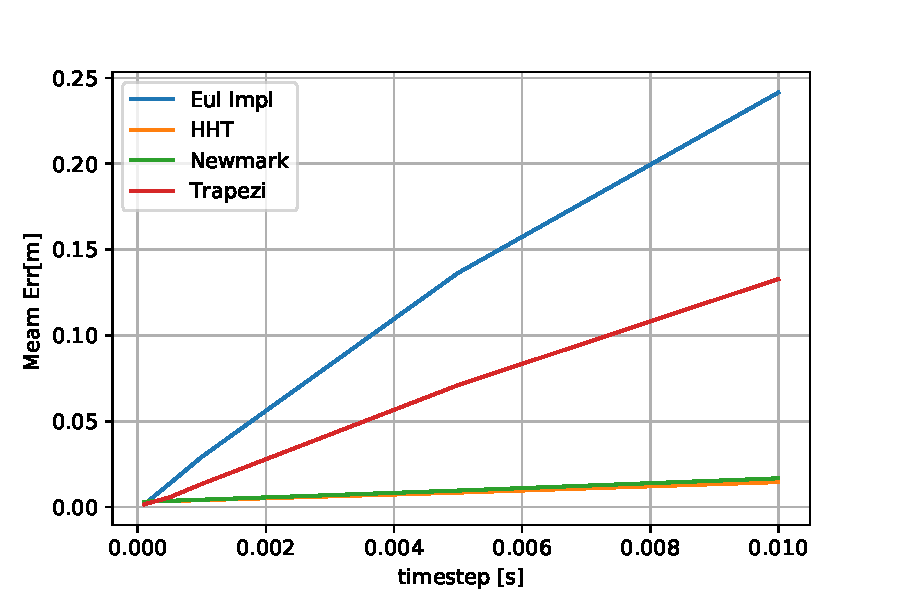
\includegraphics[height=7cm]{Figure/Convergenza/ErrComp_zoom.pdf}
\caption{Zoom Confronto Errore Medio Metodi Integrazione}
 \label{fig:ErrComp_zoom}
\end{figure}